%%____________________________________________________________________________||
\section{Results}
\label{app:results}


\subsection{\texorpdfstring{\mht}{MHT} shapes for masked fit }

\documentclass{article}
\usepackage[utf8]{inputenc}
\usepackage{rotating}
\begin{document}
\clearpage
\begin{sidewaystable}
\caption{A summary of the cumulative signal acceptance times efficiency, $\mathcal{A}\,\varepsilon$ [\%], for various benchmark models with both compressed and uncompressed mass spectra, following the application of the event selection criteria used to define the signal region. Values for $\mathcal{A}\,\varepsilon$ are also shown following the application of additional requirements that define the four most sensitive $n_{\mathrm{jet}}$ event categories, as defined in Table 5. Scale factor corrections to simulated signal events that account for the mismodelling of theoretical and experimental parameters are not applied, and so the values for $\mathcal{A}\,\varepsilon$ differ with respect to those in Table 5 by up to 15\%. }
\begin{tabular}{lcccccc}
  \hline
  Event selection & \multicolumn{6}{c}{Benchmark model ($m_\mathrm{SUSY},\,m_\mathrm{LSP}$)} \\
  \cline{2-7}
   & T1qqqq & T1qqqq & T2qq\_8fold & T2qq\_8fold & T2qq\_1fold & T2qq\_1fold \\
   & (1300,\,100) & (900,\,700) & (1050,\,100) & (650,\,550) & (600,\,50) & (400,\,250) \\
  \hline
  Before selection & 100\phantom{.1} & 100\phantom{.1} & 100\phantom{.1} & 100\phantom{.1} & 100\phantom{.1} & 100\phantom{.1} \\
  Event veto for muons and electrons & \phantom{1}99\phantom{.1} & 100\phantom{.1} & 100\phantom{.1} & 100\phantom{.1} & 100\phantom{.1} & 100\phantom{.1} \\
  Event veto for single isolated tracks & \phantom{1}94\phantom{.1} & \phantom{1}91\phantom{.1} & \phantom{1}96\phantom{.1} & \phantom{1}95\phantom{.1} & \phantom{1}96\phantom{.1} & \phantom{1}95\phantom{.1} \\
  Event veto for photons & \phantom{1}92\phantom{.1} & \phantom{1}90\phantom{.1} & \phantom{1}95\phantom{.1} & \phantom{1}94\phantom{.1} & \phantom{1}95\phantom{.1} & \phantom{1}95\phantom{.1} \\
  Event veto for forward jets ($|\eta| > 3.0$) & \phantom{1}81\phantom{.1} & \phantom{1}78\phantom{.1} & \phantom{1}82\phantom{.1} & \phantom{1}81\phantom{.1} & \phantom{1}80\phantom{.1} & \phantom{1}80\phantom{.1} \\
  $n_{\mathrm{jet}} \geq 2$ & \phantom{1}81\phantom{.1} & \phantom{1}78\phantom{.1} & \phantom{1}81\phantom{.1} & \phantom{1}72\phantom{.1} & \phantom{1}80\phantom{.1} & \phantom{1}75\phantom{.1} \\
  $p_{\mathrm{T}}^{\mathrm{j_1}} > 100\,\mathrm{GeV}$ & \phantom{1}81\phantom{.1} & \phantom{1}71\phantom{.1} & \phantom{1}81\phantom{.1} & \phantom{1}57\phantom{.1} & \phantom{1}79\phantom{.1} & \phantom{1}66\phantom{.1} \\
  $|\eta^{\mathrm{j_1}}| < 2.5$ & \phantom{1}81\phantom{.1} & \phantom{1}70\phantom{.1} & \phantom{1}81\phantom{.1} & \phantom{1}55\phantom{.1} & \phantom{1}79\phantom{.1} & \phantom{1}65\phantom{.1} \\
  $H_{\mathrm{T}} > 200\,\mathrm{GeV}$ & \phantom{1}81\phantom{.1} & \phantom{1}69\phantom{.1} & \phantom{1}81\phantom{.1} & \phantom{1}50\phantom{.1} & \phantom{1}79\phantom{.1} & \phantom{1}60\phantom{.1} \\
  $H_{\mathrm{T}}^{\mathrm{miss}} > 130\,\mathrm{GeV}$ & \phantom{1}77\phantom{.1} & \phantom{1}50\phantom{.1} & \phantom{1}78\phantom{.1} & \phantom{1}33\phantom{.1} & \phantom{1}71\phantom{.1} & \phantom{1}40\phantom{.1} \\
  $H_{\mathrm{T}}^{\mathrm{miss}} / E_{\mathrm{T}}^{\mathrm{miss}} < 1.25$ & \phantom{1}74\phantom{.1} & \phantom{1}44\phantom{.1} & \phantom{1}75\phantom{.1} & \phantom{1}28\phantom{.1} & \phantom{1}65\phantom{.1} & \phantom{1}33\phantom{.1} \\
  $H_{\mathrm{T}}$-dependent $\alpha_{\mathrm{T}}$ requirements ($H_{\mathrm{T}} < 800\,\mathrm{GeV}$) & \phantom{1}74\phantom{.1} & \phantom{1}30\phantom{.1} & \phantom{1}71\phantom{.1} & \phantom{1}15\phantom{.1} & \phantom{1}50\phantom{.1} & \phantom{1}17\phantom{.1} \\
  $\Delta\phi^{*}_{\mathrm{min}} > 0.5$ & \phantom{1}22\phantom{.1} & \phantom{1}18\phantom{.1} & \phantom{1}44\phantom{.1} & \phantom{1}10\phantom{.1} & \phantom{1}33\phantom{.1} & \phantom{1}13\phantom{.1} \\
  \hline
  Four most sensitive $n_{\mathrm{jet}}$ event categories & \phantom{1}22\phantom{.1} & \phantom{1}13\phantom{.1} & \phantom{1}43\phantom{.1} & \phantom{10}5.5 & \phantom{1}31\phantom{.1} & \phantom{10}6.1 \\
  \hline
\end{tabular}
\end{sidewaystable}

\clearpage
\begin{sidewaystable}
\caption{A summary of the cumulative signal acceptance times efficiency, $\mathcal{A}\,\varepsilon$ [\%], for various benchmark models with both compressed and uncompressed mass spectra, following the application of the event selection criteria used to define the signal region. Values for $\mathcal{A}\,\varepsilon$ are also shown following the application of additional requirements that define the four most sensitive $n_{\mathrm{jet}}$ event categories, as defined in Table 5. Scale factor corrections to simulated signal events that account for the mismodelling of theoretical and experimental parameters are not applied, and so the values for $\mathcal{A}\,\varepsilon$ differ with respect to those in Table 5 by up to 15\%. }
\begin{tabular}{lcccccc}
  \hline
  Event selection & \multicolumn{6}{c}{Benchmark model ($m_\mathrm{SUSY},\,m_\mathrm{LSP}$)} \\
  \cline{2-7}
   & T1bbbb & T1bbbb & T1tttt & T1tttt & T1ttbb & T1ttbb \\
   & (1500,\,100) & (1000,\,800) & (1300,\,100) & (800,\,400) & (1300,\,100) & (1000,\,700) \\
  \hline
  Before selection & 100\phantom{.1} & 100\phantom{.1} & 100\phantom{.1} & 100\phantom{.1} & 100\phantom{.1} & 100\phantom{.1} \\
  Event veto for muons and electrons & \phantom{1}99\phantom{.1} & \phantom{1}98\phantom{.1} & \phantom{1}41\phantom{.1} & \phantom{1}42\phantom{.1} & \phantom{1}61\phantom{.1} & \phantom{1}64\phantom{.1} \\
  Event veto for single isolated tracks & \phantom{1}94\phantom{.1} & \phantom{1}91\phantom{.1} & \phantom{1}31\phantom{.1} & \phantom{1}32\phantom{.1} & \phantom{1}51\phantom{.1} & \phantom{1}54\phantom{.1} \\
  Event veto for photons & \phantom{1}93\phantom{.1} & \phantom{1}91\phantom{.1} & \phantom{1}30\phantom{.1} & \phantom{1}32\phantom{.1} & \phantom{1}50\phantom{.1} & \phantom{1}54\phantom{.1} \\
  Event veto for forward jets ($|\eta| > 3.0$) & \phantom{1}82\phantom{.1} & \phantom{1}79\phantom{.1} & \phantom{1}27\phantom{.1} & \phantom{1}27\phantom{.1} & \phantom{1}44\phantom{.1} & \phantom{1}47\phantom{.1} \\
  $n_{\mathrm{jet}} \geq 2$ & \phantom{1}82\phantom{.1} & \phantom{1}78\phantom{.1} & \phantom{1}27\phantom{.1} & \phantom{1}27\phantom{.1} & \phantom{1}44\phantom{.1} & \phantom{1}47\phantom{.1} \\
  $p_{\mathrm{T}}^{\mathrm{j_1}} > 100\,\mathrm{GeV}$ & \phantom{1}82\phantom{.1} & \phantom{1}69\phantom{.1} & \phantom{1}27\phantom{.1} & \phantom{1}25\phantom{.1} & \phantom{1}44\phantom{.1} & \phantom{1}43\phantom{.1} \\
  $|\eta^{\mathrm{j_1}}| < 2.5$ & \phantom{1}82\phantom{.1} & \phantom{1}68\phantom{.1} & \phantom{1}27\phantom{.1} & \phantom{1}25\phantom{.1} & \phantom{1}44\phantom{.1} & \phantom{1}42\phantom{.1} \\
  $H_{\mathrm{T}} > 200\,\mathrm{GeV}$ & \phantom{1}82\phantom{.1} & \phantom{1}66\phantom{.1} & \phantom{1}27\phantom{.1} & \phantom{1}25\phantom{.1} & \phantom{1}44\phantom{.1} & \phantom{1}42\phantom{.1} \\
  $H_{\mathrm{T}}^{\mathrm{miss}} > 130\,\mathrm{GeV}$ & \phantom{1}79\phantom{.1} & \phantom{1}48\phantom{.1} & \phantom{1}25\phantom{.1} & \phantom{1}15\phantom{.1} & \phantom{1}41\phantom{.1} & \phantom{1}32\phantom{.1} \\
  $H_{\mathrm{T}}^{\mathrm{miss}} / E_{\mathrm{T}}^{\mathrm{miss}} < 1.25$ & \phantom{1}77\phantom{.1} & \phantom{1}43\phantom{.1} & \phantom{1}24\phantom{.1} & \phantom{1}11\phantom{.1} & \phantom{1}38\phantom{.1} & \phantom{1}26\phantom{.1} \\
  $H_{\mathrm{T}}$-dependent $\alpha_{\mathrm{T}}$ requirements ($H_{\mathrm{T}} < 800\,\mathrm{GeV}$) & \phantom{1}77\phantom{.1} & \phantom{1}29\phantom{.1} & \phantom{1}24\phantom{.1} & \phantom{10}8.3 & \phantom{1}38\phantom{.1} & \phantom{1}19\phantom{.1} \\
  $\Delta\phi^{*}_{\mathrm{min}} > 0.5$ & \phantom{1}23\phantom{.1} & \phantom{1}17\phantom{.1} & \phantom{10}5.6 & \phantom{10}1.3 & \phantom{10}9.5 & \phantom{10}8.8 \\
  \hline
  Four most sensitive $n_{\mathrm{jet}}$ event categories & \phantom{1}23\phantom{.1} & \phantom{1}12\phantom{.1} & \phantom{10}5.6 & \phantom{10}1.3 & \phantom{10}9.5 & \phantom{10}7.4 \\
  \hline
\end{tabular}
\end{sidewaystable}

\clearpage
\begin{sidewaystable}
\caption{A summary of the cumulative signal acceptance times efficiency, $\mathcal{A}\,\varepsilon$ [\%], for various benchmark models with both compressed and uncompressed mass spectra, following the application of the event selection criteria used to define the signal region. Values for $\mathcal{A}\,\varepsilon$ are also shown following the application of additional requirements that define the four most sensitive $n_{\mathrm{jet}}$ event categories, as defined in Table 5. Scale factor corrections to simulated signal events that account for the mismodelling of theoretical and experimental parameters are not applied, and so the values for $\mathcal{A}\,\varepsilon$ differ with respect to those in Table 5 by up to 15\%. }
\begin{tabular}{lcccc}
  \hline
  Event selection & \multicolumn{4}{c}{Benchmark model ($m_\mathrm{SUSY},\,m_\mathrm{LSP}$)} \\
  \cline{2-5}
   & T5tttt\_DM175 & T5tttt\_DM175 & T5ttcc & T5ttcc \\
   & (800,\,100) & (700,\,400) & (1200,\,200) & (750,\,600) \\
  \hline
  Before selection & 100\phantom{.1} & 100\phantom{.1} & 100\phantom{.1} & 100\phantom{.1} \\
  Event veto for muons and electrons & \phantom{1}41\phantom{.1} & \phantom{1}42\phantom{.1} & \phantom{1}63\phantom{.1} & \phantom{1}63\phantom{.1} \\
  Event veto for single isolated tracks & \phantom{1}30\phantom{.1} & \phantom{1}32\phantom{.1} & \phantom{1}53\phantom{.1} & \phantom{1}53\phantom{.1} \\
  Event veto for photons & \phantom{1}30\phantom{.1} & \phantom{1}31\phantom{.1} & \phantom{1}53\phantom{.1} & \phantom{1}52\phantom{.1} \\
  Event veto for forward jets ($|\eta| > 3.0$) & \phantom{1}25\phantom{.1} & \phantom{1}27\phantom{.1} & \phantom{1}46\phantom{.1} & \phantom{1}45\phantom{.1} \\
  $n_{\mathrm{jet}} \geq 2$ & \phantom{1}25\phantom{.1} & \phantom{1}27\phantom{.1} & \phantom{1}46\phantom{.1} & \phantom{1}41\phantom{.1} \\
  $p_{\mathrm{T}}^{\mathrm{j_1}} > 100\,\mathrm{GeV}$ & \phantom{1}25\phantom{.1} & \phantom{1}21\phantom{.1} & \phantom{1}46\phantom{.1} & \phantom{1}25\phantom{.1} \\
  $|\eta^{\mathrm{j_1}}| < 2.5$ & \phantom{1}25\phantom{.1} & \phantom{1}21\phantom{.1} & \phantom{1}46\phantom{.1} & \phantom{1}24\phantom{.1} \\
  $H_{\mathrm{T}} > 200\,\mathrm{GeV}$ & \phantom{1}25\phantom{.1} & \phantom{1}21\phantom{.1} & \phantom{1}46\phantom{.1} & \phantom{1}23\phantom{.1} \\
  $H_{\mathrm{T}}^{\mathrm{miss}} > 130\,\mathrm{GeV}$ & \phantom{1}17\phantom{.1} & \phantom{10}9.4 & \phantom{1}44\phantom{.1} & \phantom{1}15\phantom{.1} \\
  $H_{\mathrm{T}}^{\mathrm{miss}} / E_{\mathrm{T}}^{\mathrm{miss}} < 1.25$ & \phantom{1}11\phantom{.1} & \phantom{10}5.6 & \phantom{1}42\phantom{.1} & \phantom{1}12\phantom{.1} \\
  $H_{\mathrm{T}}$-dependent $\alpha_{\mathrm{T}}$ requirements ($H_{\mathrm{T}} < 800\,\mathrm{GeV}$) & \phantom{1}11\phantom{.1} & \phantom{10}3.9 & \phantom{1}41\phantom{.1} & \phantom{10}7.5 \\
  $\Delta\phi^{*}_{\mathrm{min}} > 0.5$ & \phantom{10}0.4 & \phantom{10}0.5 & \phantom{1}13\phantom{.1} & \phantom{10}3.2 \\
  \hline
  Four most sensitive $n_{\mathrm{jet}}$ event categories & \phantom{10}0.4 & \phantom{10}0.4 & \phantom{1}13\phantom{.1} & \phantom{10}2.3 \\
  \hline
\end{tabular}
\end{sidewaystable}

\clearpage
\begin{sidewaystable}
\caption{A summary of the cumulative signal acceptance times efficiency, $\mathcal{A}\,\varepsilon$ [\%], for various benchmark models with both compressed and uncompressed mass spectra, following the application of the event selection criteria used to define the signal region. Values for $\mathcal{A}\,\varepsilon$ are also shown following the application of additional requirements that define the four most sensitive $n_{\mathrm{jet}}$ event categories, as defined in Table 5. Scale factor corrections to simulated signal events that account for the mismodelling of theoretical and experimental parameters are not applied, and so the values for $\mathcal{A}\,\varepsilon$ differ with respect to those in Table 5 by up to 15\%. }
\begin{tabular}{lcccccc}
  \hline
  Event selection & \multicolumn{6}{c}{Benchmark model ($m_\mathrm{SUSY},\,m_\mathrm{LSP}$)} \\
  \cline{2-7}
   & T2bb & T2bb & T2tb & T2tb & T2tt & T2tt \\
   & (800,\,50) & (375,\,300) & (600,\,50) & (350,\,225) & (700,\,50) & (350,\,100) \\
  \hline
  Before selection & 100\phantom{.1} & 100\phantom{.1} & 100\phantom{.1} & 100\phantom{.1} & 100\phantom{.1} & 100\phantom{.1} \\
  Event veto for muons and electrons & \phantom{1}99\phantom{.1} & \phantom{1}99\phantom{.1} & \phantom{1}72\phantom{.1} & \phantom{1}80\phantom{.1} & \phantom{1}63\phantom{.1} & \phantom{1}63\phantom{.1} \\
  Event veto for single isolated tracks & \phantom{1}96\phantom{.1} & \phantom{1}94\phantom{.1} & \phantom{1}61\phantom{.1} & \phantom{1}72\phantom{.1} & \phantom{1}53\phantom{.1} & \phantom{1}53\phantom{.1} \\
  Event veto for photons & \phantom{1}95\phantom{.1} & \phantom{1}94\phantom{.1} & \phantom{1}60\phantom{.1} & \phantom{1}72\phantom{.1} & \phantom{1}52\phantom{.1} & \phantom{1}52\phantom{.1} \\
  Event veto for forward jets ($|\eta| > 3.0$) & \phantom{1}81\phantom{.1} & \phantom{1}81\phantom{.1} & \phantom{1}51\phantom{.1} & \phantom{1}62\phantom{.1} & \phantom{1}45\phantom{.1} & \phantom{1}45\phantom{.1} \\
  $n_{\mathrm{jet}} \geq 2$ & \phantom{1}80\phantom{.1} & \phantom{1}61\phantom{.1} & \phantom{1}51\phantom{.1} & \phantom{1}53\phantom{.1} & \phantom{1}45\phantom{.1} & \phantom{1}44\phantom{.1} \\
  $p_{\mathrm{T}}^{\mathrm{j_1}} > 100\,\mathrm{GeV}$ & \phantom{1}80\phantom{.1} & \phantom{1}36\phantom{.1} & \phantom{1}50\phantom{.1} & \phantom{1}36\phantom{.1} & \phantom{1}44\phantom{.1} & \phantom{1}35\phantom{.1} \\
  $|\eta^{\mathrm{j_1}}| < 2.5$ & \phantom{1}80\phantom{.1} & \phantom{1}34\phantom{.1} & \phantom{1}50\phantom{.1} & \phantom{1}34\phantom{.1} & \phantom{1}44\phantom{.1} & \phantom{1}34\phantom{.1} \\
  $H_{\mathrm{T}} > 200\,\mathrm{GeV}$ & \phantom{1}80\phantom{.1} & \phantom{1}30\phantom{.1} & \phantom{1}50\phantom{.1} & \phantom{1}30\phantom{.1} & \phantom{1}44\phantom{.1} & \phantom{1}33\phantom{.1} \\
  $H_{\mathrm{T}}^{\mathrm{miss}} > 130\,\mathrm{GeV}$ & \phantom{1}75\phantom{.1} & \phantom{1}18\phantom{.1} & \phantom{1}44\phantom{.1} & \phantom{1}17\phantom{.1} & \phantom{1}40\phantom{.1} & \phantom{1}20\phantom{.1} \\
  $H_{\mathrm{T}}^{\mathrm{miss}} / E_{\mathrm{T}}^{\mathrm{miss}} < 1.25$ & \phantom{1}72\phantom{.1} & \phantom{1}15\phantom{.1} & \phantom{1}38\phantom{.1} & \phantom{1}12\phantom{.1} & \phantom{1}38\phantom{.1} & \phantom{1}15\phantom{.1} \\
  $H_{\mathrm{T}}$-dependent $\alpha_{\mathrm{T}}$ requirements ($H_{\mathrm{T}} < 800\,\mathrm{GeV}$) & \phantom{1}62\phantom{.1} & \phantom{10}7.2 & \phantom{1}30\phantom{.1} & \phantom{10}5.5 & \phantom{1}34\phantom{.1} & \phantom{10}8.8 \\
  $\Delta\phi^{*}_{\mathrm{min}} > 0.5$ & \phantom{1}39\phantom{.1} & \phantom{10}4.5 & \phantom{1}17\phantom{.1} & \phantom{10}3.2 & \phantom{1}21\phantom{.1} & \phantom{10}4.0 \\
  \hline
  Four most sensitive $n_{\mathrm{jet}}$ event categories & \phantom{1}37\phantom{.1} & \phantom{10}2.9 & \phantom{1}14\phantom{.1} & \phantom{10}2.1 & \phantom{1}19\phantom{.1} & \phantom{10}3.0 \\
  \hline
\end{tabular}
\end{sidewaystable}

\clearpage
\begin{sidewaystable}
\caption{A summary of the cumulative signal acceptance times efficiency, $\mathcal{A}\,\varepsilon$ [\%], for various benchmark models with both compressed and uncompressed mass spectra, following the application of the event selection criteria used to define the signal region. Values for $\mathcal{A}\,\varepsilon$ are also shown following the application of additional requirements that define the four most sensitive $n_{\mathrm{jet}}$ event categories, as defined in Table 5. Scale factor corrections to simulated signal events that account for the mismodelling of theoretical and experimental parameters are not applied, and so the values for $\mathcal{A}\,\varepsilon$ differ with respect to those in Table 5 by up to 15\%. }
\begin{tabular}{lccc}
  \hline
  Event selection & \multicolumn{3}{c}{Benchmark model ($m_\mathrm{SUSY},\,m_\mathrm{LSP}$)} \\
  \cline{2-4}
   & T2cc & T2tt\_degen & T2tt\_mixed \\
   & (325,\,305) & (300,\,290) & (300,\,250) \\
  \hline
  Before selection & 100\phantom{.1} & 100\phantom{.1} & 100\phantom{.1} \\
  Event veto for muons and electrons & 100\phantom{.1} & 100\phantom{.1} & \phantom{1}89\phantom{.1} \\
  Event veto for single isolated tracks & \phantom{1}97\phantom{.1} & \phantom{1}98\phantom{.1} & \phantom{1}83\phantom{.1} \\
  Event veto for photons & \phantom{1}97\phantom{.1} & \phantom{1}97\phantom{.1} & \phantom{1}83\phantom{.1} \\
  Event veto for forward jets ($|\eta| > 3.0$) & \phantom{1}83\phantom{.1} & \phantom{1}84\phantom{.1} & \phantom{1}72\phantom{.1} \\
  $n_{\mathrm{jet}} \geq 2$ & \phantom{1}26\phantom{.1} & \phantom{1}21\phantom{.1} & \phantom{1}36\phantom{.1} \\
  $p_{\mathrm{T}}^{\mathrm{j_1}} > 100\,\mathrm{GeV}$ & \phantom{1}16\phantom{.1} & \phantom{1}14\phantom{.1} & \phantom{1}19\phantom{.1} \\
  $|\eta^{\mathrm{j_1}}| < 2.5$ & \phantom{1}15\phantom{.1} & \phantom{1}13\phantom{.1} & \phantom{1}18\phantom{.1} \\
  $H_{\mathrm{T}} > 200\,\mathrm{GeV}$ & \phantom{1}13\phantom{.1} & \phantom{1}11\phantom{.1} & \phantom{1}15\phantom{.1} \\
  $H_{\mathrm{T}}^{\mathrm{miss}} > 130\,\mathrm{GeV}$ & \phantom{1}11\phantom{.1} & \phantom{10}9.2 & \phantom{1}10\phantom{.1} \\
  $H_{\mathrm{T}}^{\mathrm{miss}} / E_{\mathrm{T}}^{\mathrm{miss}} < 1.25$ & \phantom{10}9.2 & \phantom{10}7.5 & \phantom{10}8.4 \\
  $H_{\mathrm{T}}$-dependent $\alpha_{\mathrm{T}}$ requirements ($H_{\mathrm{T}} < 800\,\mathrm{GeV}$) & \phantom{10}4.8 & \phantom{10}4.3 & \phantom{10}3.7 \\
  $\Delta\phi^{*}_{\mathrm{min}} > 0.5$ & \phantom{10}3.7 & \phantom{10}3.7 & \phantom{10}2.3 \\
  \hline
  Four most sensitive $n_{\mathrm{jet}}$ event categories & \phantom{10}1.9 & \phantom{10}1.9 & \phantom{10}0.9 \\
  \hline
\end{tabular}
\end{sidewaystable}

\end{document}

\clearpage
\subsection{Masked fit nuisance parameters}
\label{app:nuis_pre}

\begin{figure}[h!]
  \centering
  \caption{Rate parameters}
  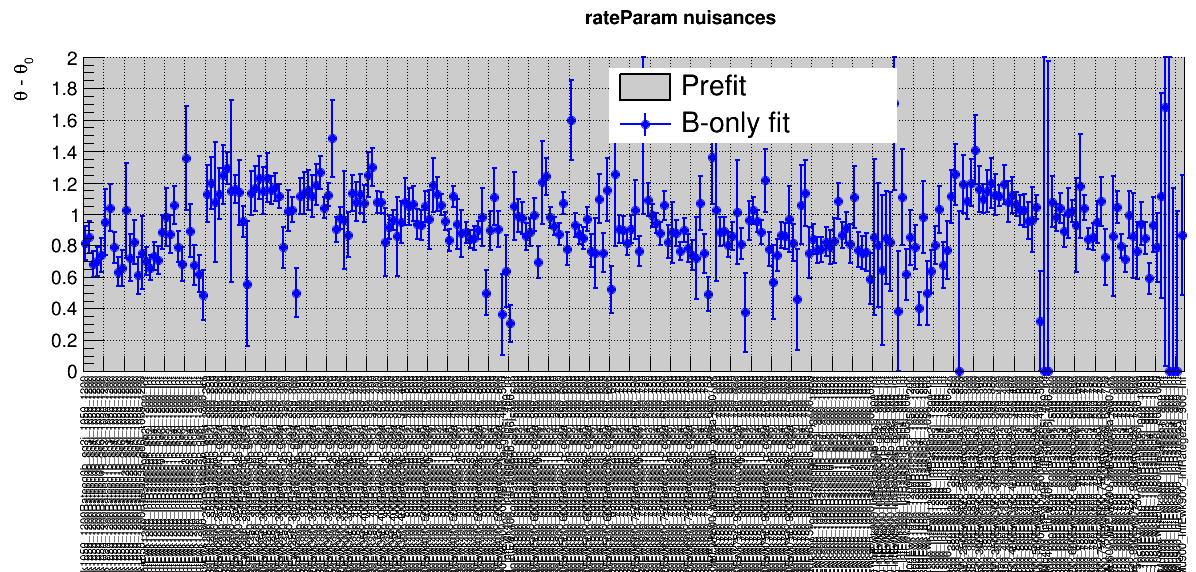
\includegraphics[width=1.\linewidth]{figures/results/prefit/nuis/Rates_nuisances}
\end{figure}

\begin{figure}[h!]
  \centering
  \caption{Correlated sources of uncertainty}
  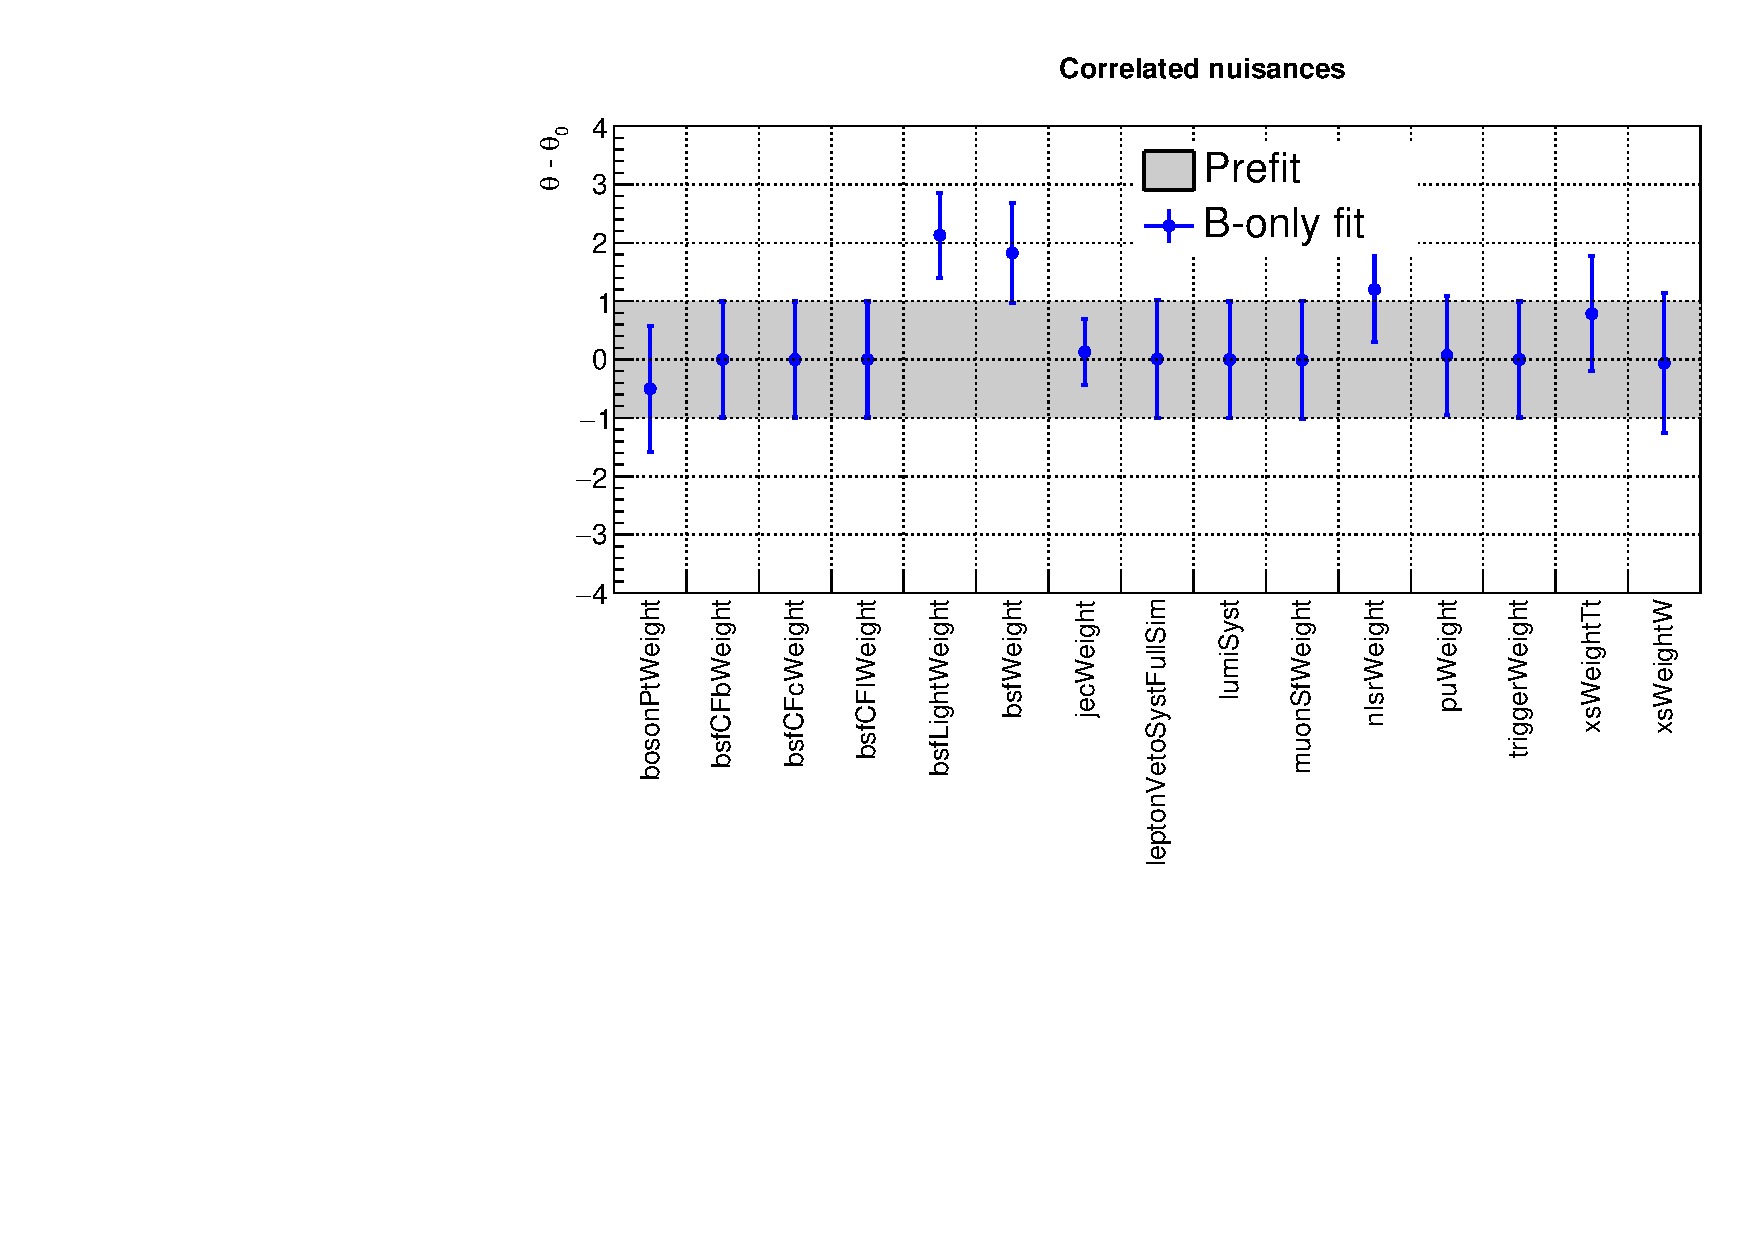
\includegraphics[width=1.\linewidth]{figures/results/prefit/nuis/Correlated_nuisances}
\end{figure}

\clearpage
\subsection{Full fit nuisance parameters}
\label{app:nuis_post}

\vspace{0.75cm} 
\begin{figure}[h!]
  \centering
  \caption{Rate parameters}
  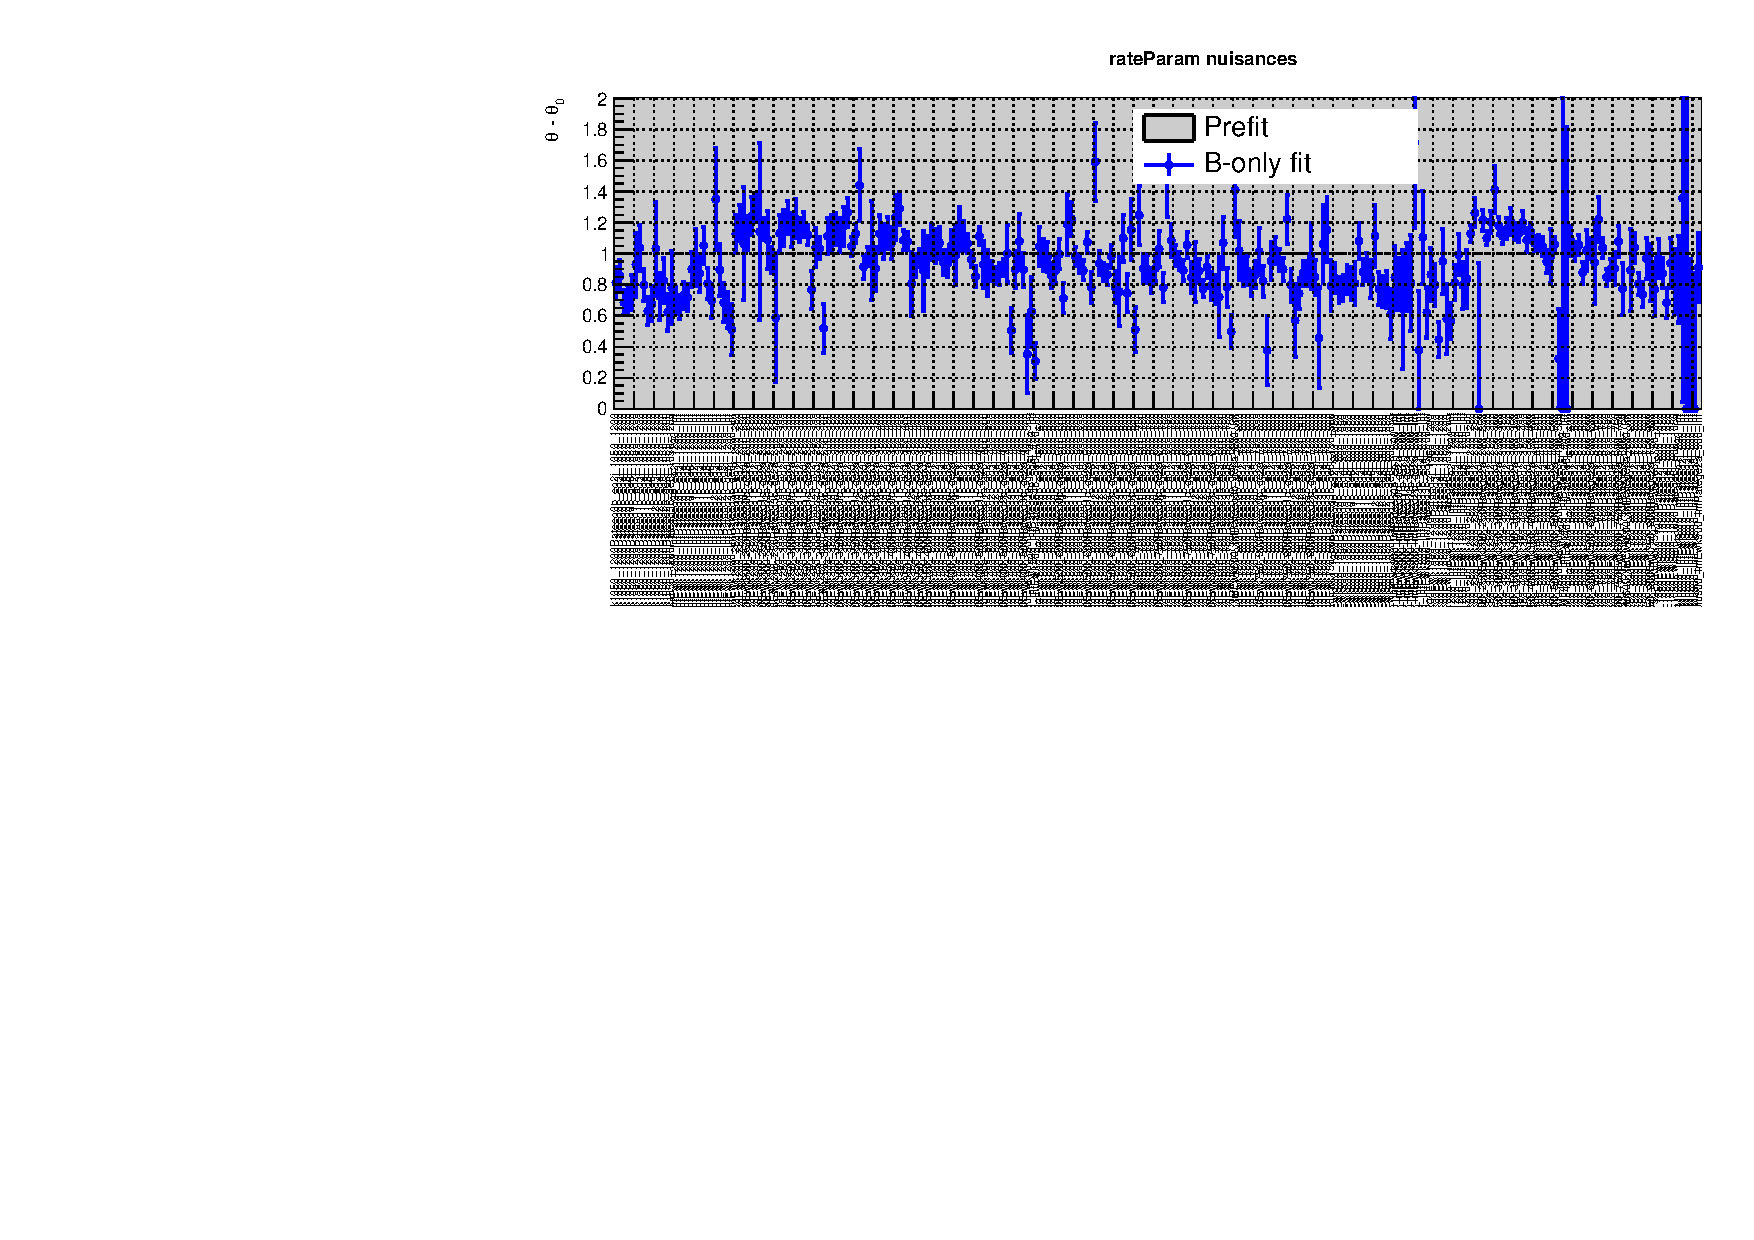
\includegraphics[width=1.\linewidth]{figures/results/postfit/nuis/Rates_nuisances}
\end{figure}

\begin{figure}[h!]
  \centering
  \caption{Correlated sources of uncertainty}
  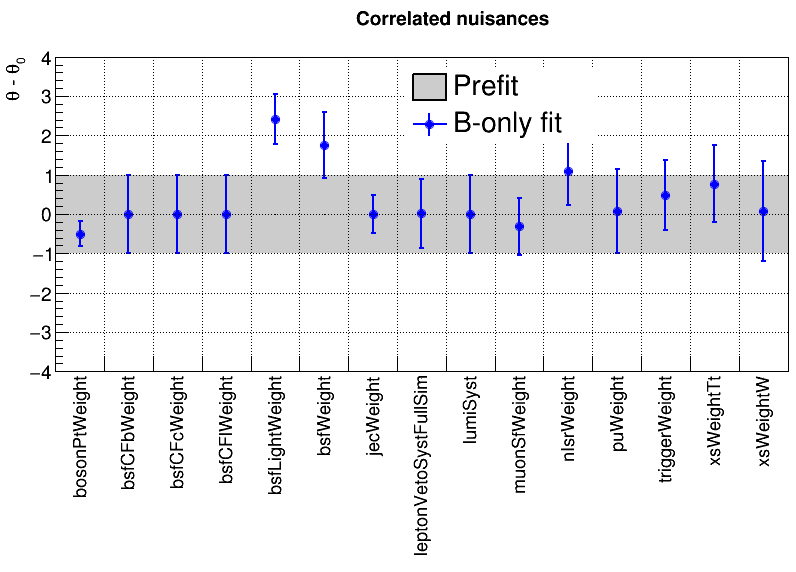
\includegraphics[width=1.\linewidth]{figures/results/postfit/nuis/Correlated_nuisances}
\end{figure}

\clearpage
\begin{figure}[h!]
  \centering
  \caption{``MC stat.'' uncertainties for lost lepton background.}
  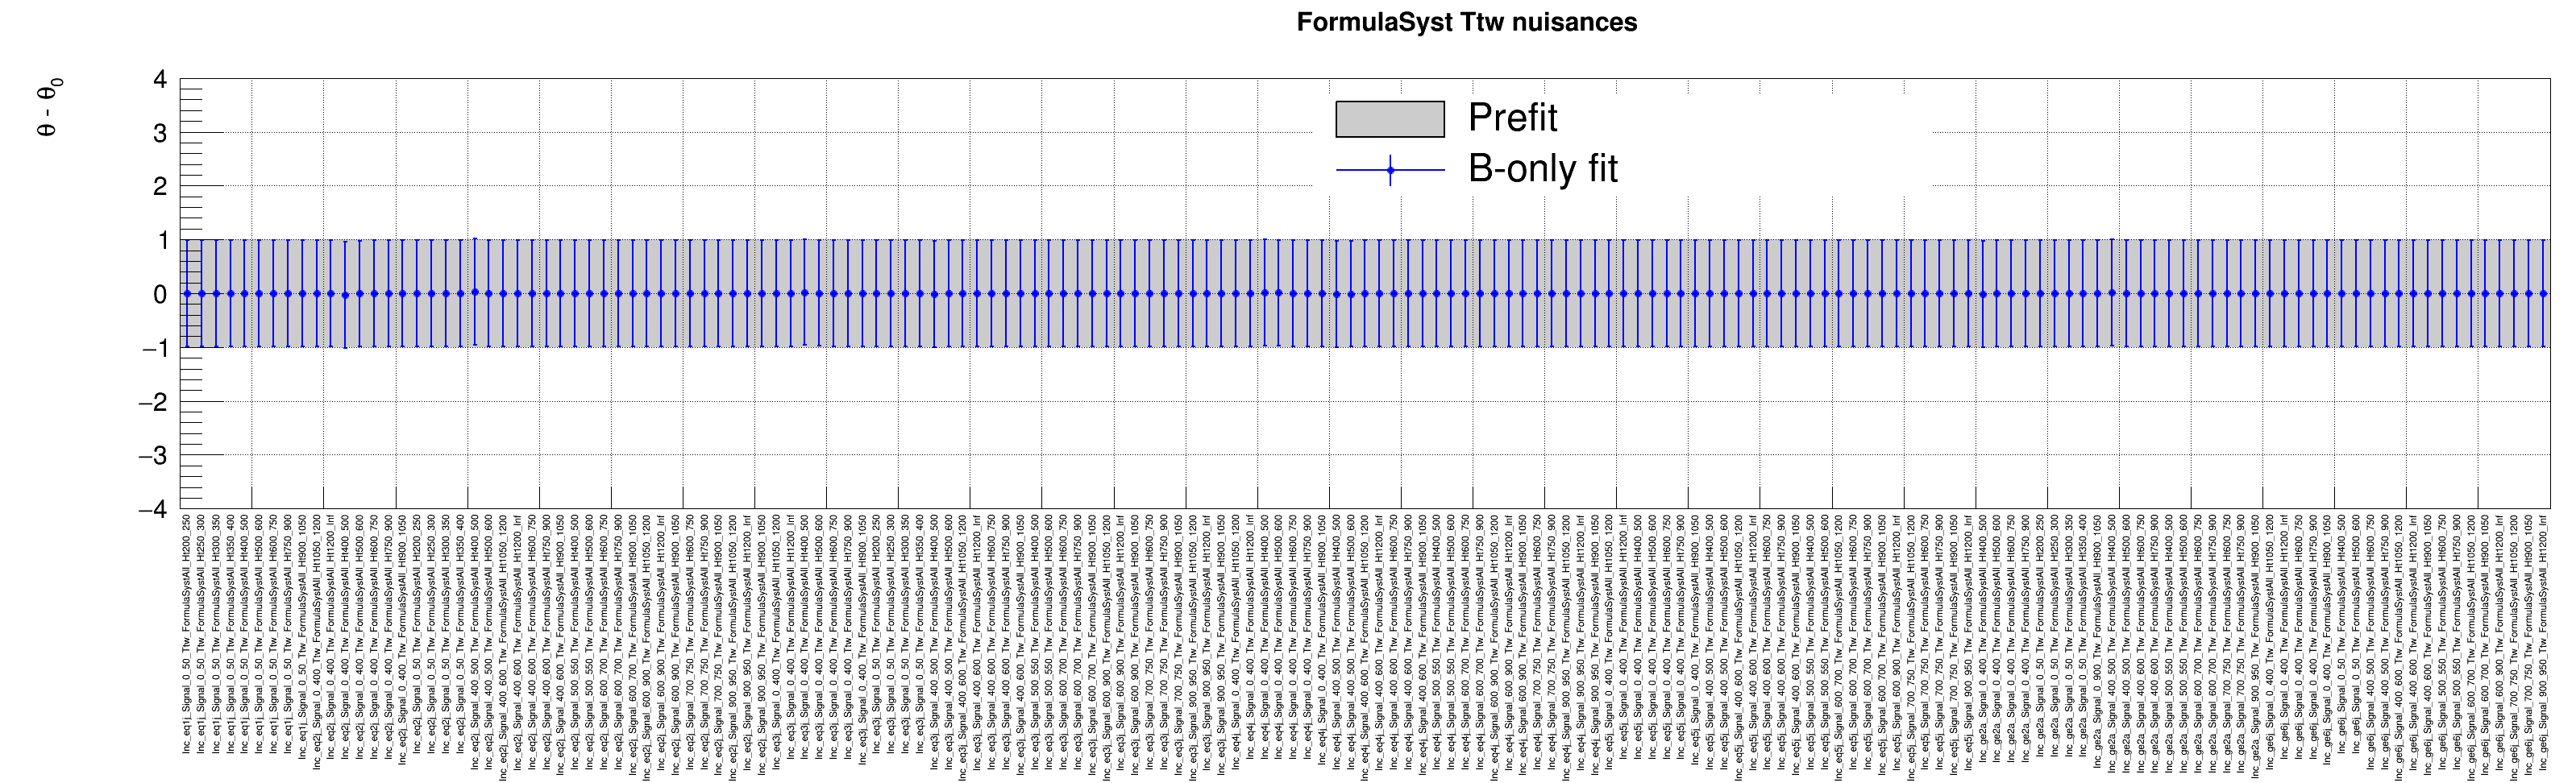
\includegraphics[width=1.\linewidth]{figures/results/postfit/nuis/FormulaSystTtw_nuisances}
\end{figure}

\begin{figure}[h!]
  \centering
  \caption{``MC stat.'' uncertainties for \znunuj background.}
  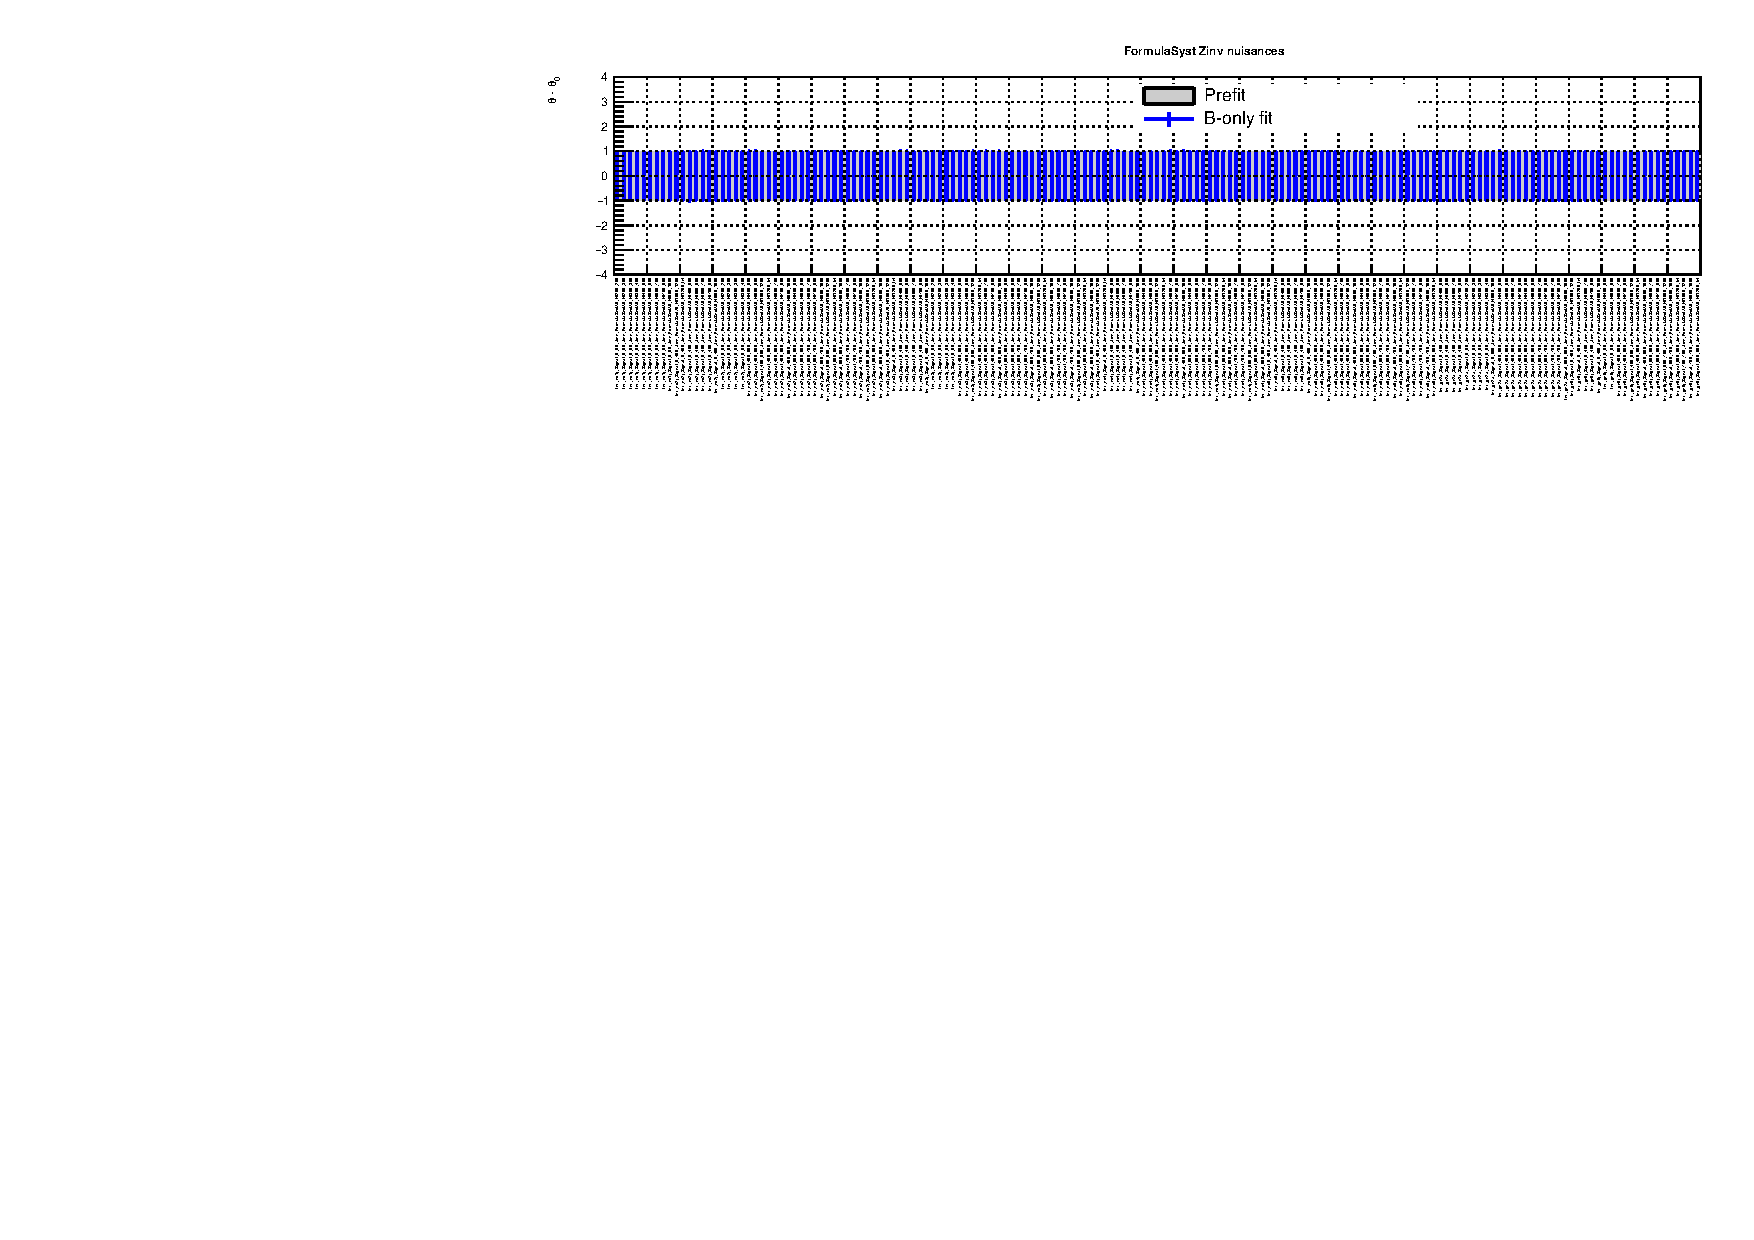
\includegraphics[width=1.\linewidth]{figures/results/postfit/nuis/FormulaSystZinv_nuisances}
\end{figure}

\clearpage
\begin{figure}[h!]
  \centering
  \caption{Systematic uncertainties in QCD background estimate}
  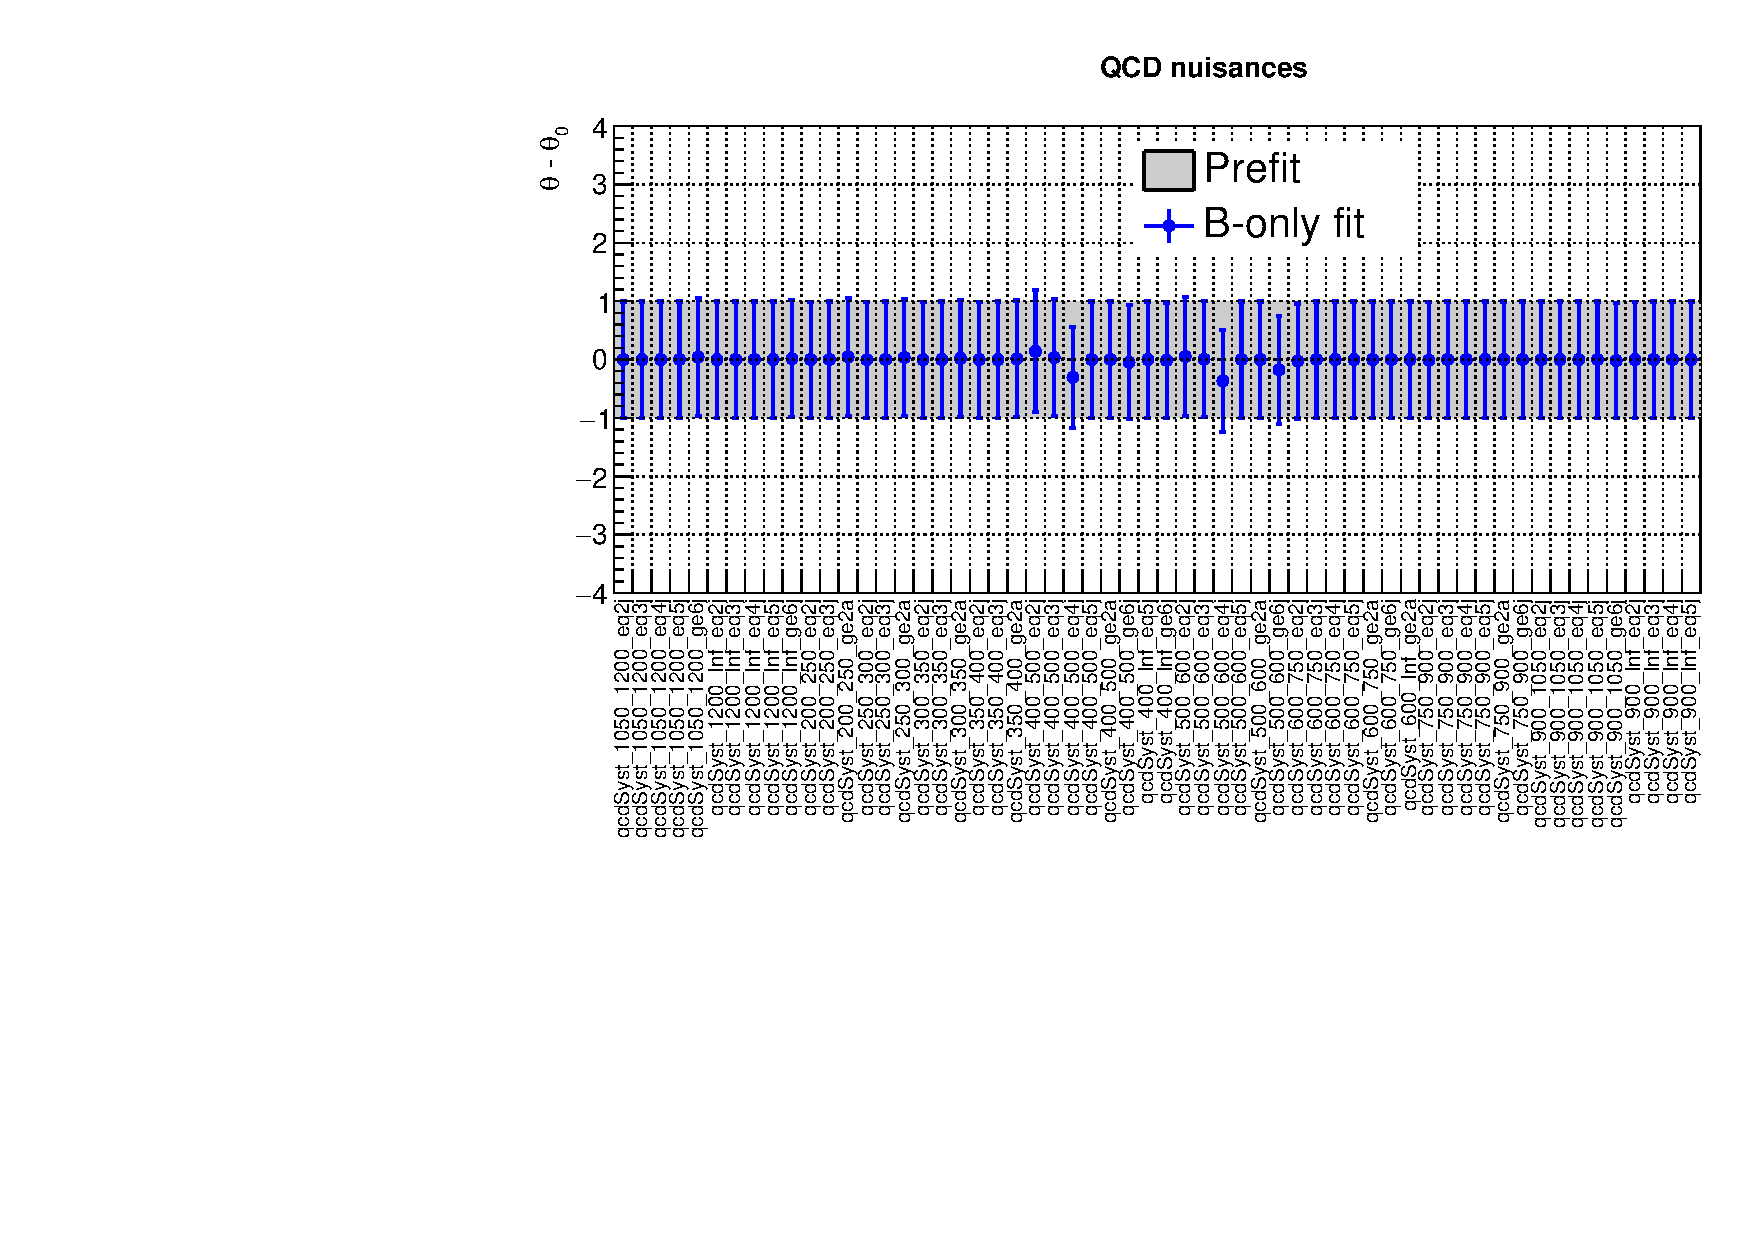
\includegraphics[width=1.\linewidth]{figures/results/postfit/nuis/qcd_nuisances}
\end{figure}

\clearpage
\begin{figure}[h!]
  \centering
  \caption{Systematic uncertainties per \scalht category in \mht modelling for lost lepton background}
  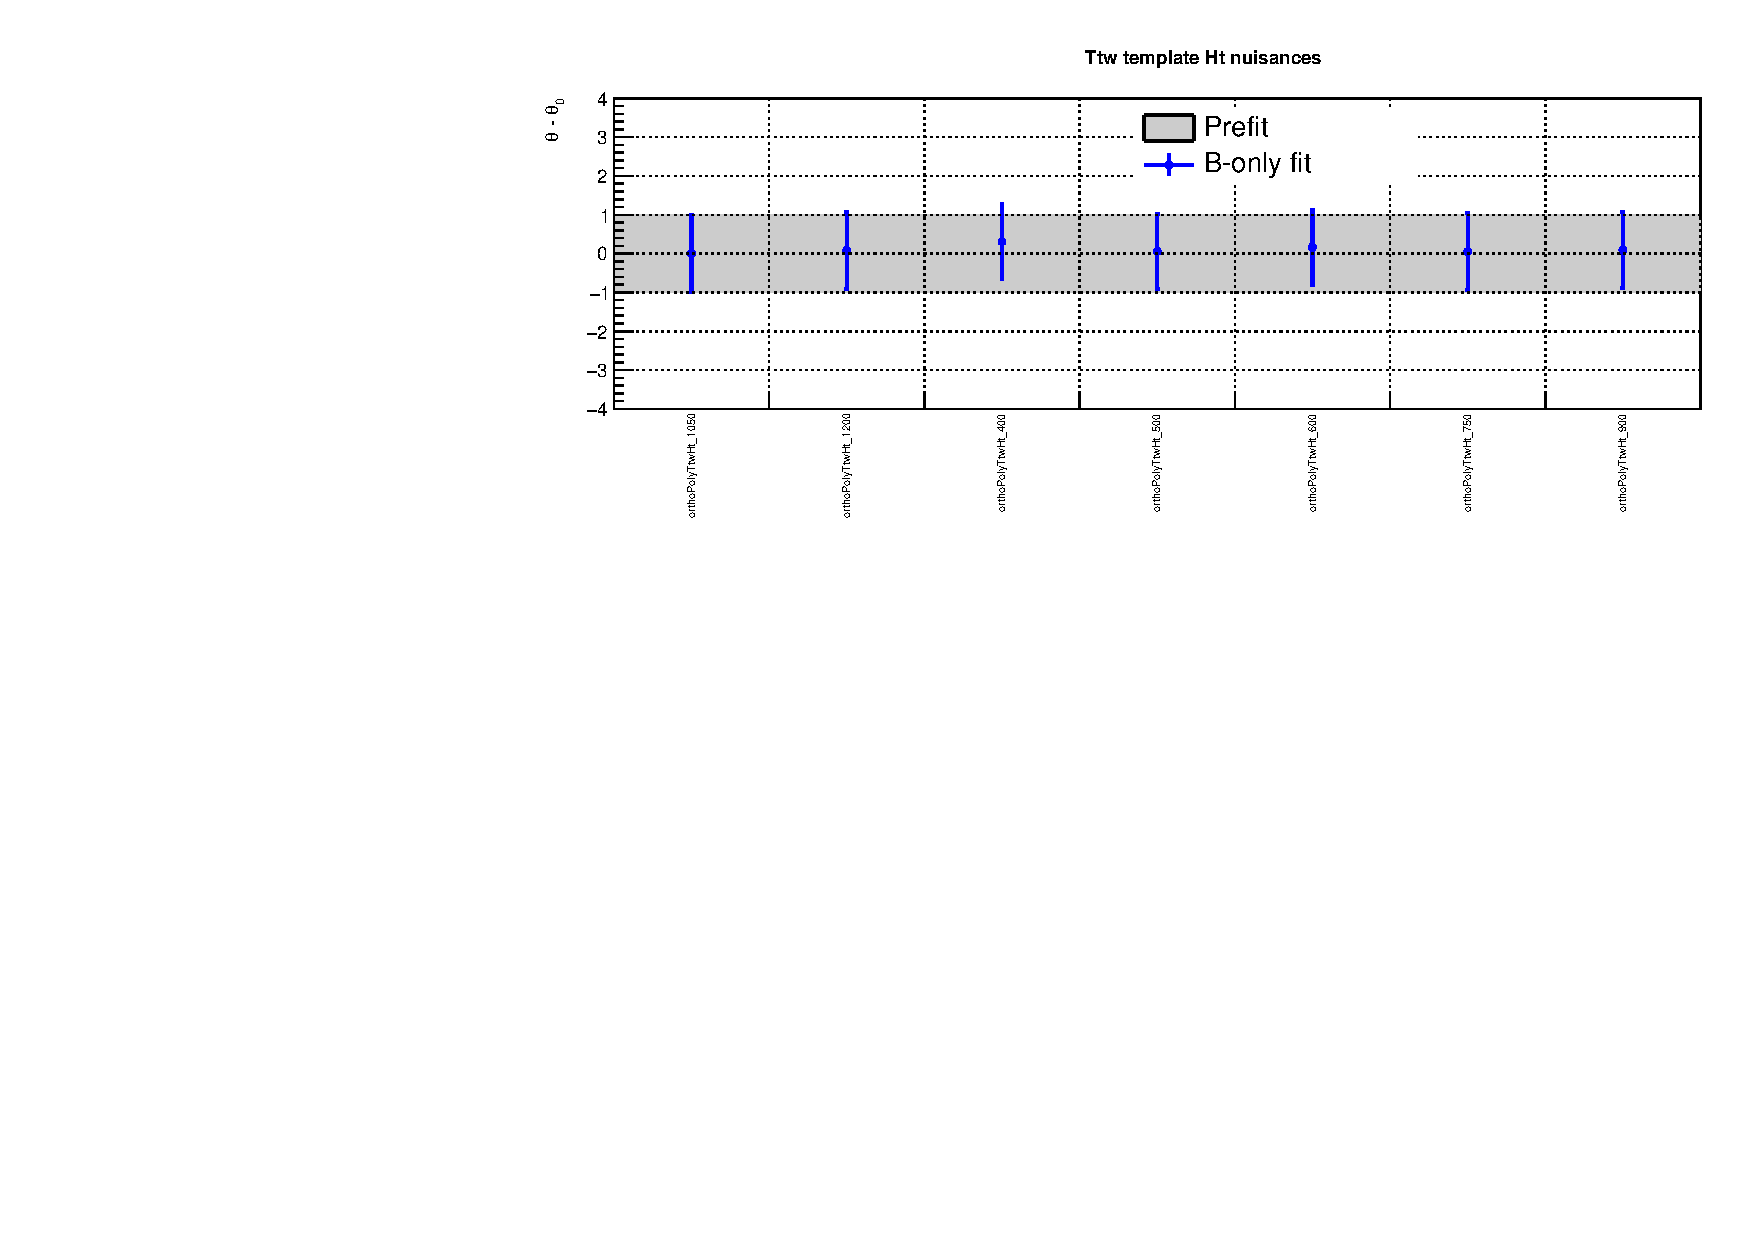
\includegraphics[width=1.\linewidth]{figures/results/postfit/nuis/TemplateTtw_ht_nuisances}
\end{figure}

\begin{figure}[h!]
  \centering
  \caption{Systematic uncertainties per \njet category in \mht modelling for lost lepton background}
  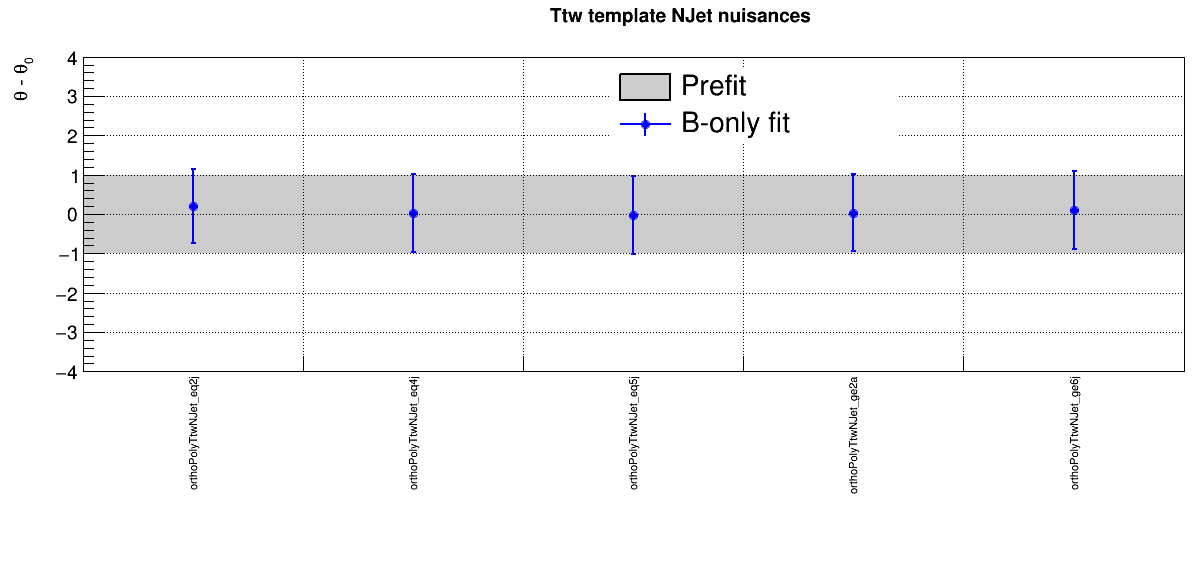
\includegraphics[width=1.\linewidth]{figures/results/postfit/nuis/TemplateTtw_njet_nuisances}
\end{figure}

\clearpage
\begin{figure}[h!]
  \centering
  \caption{Systematic uncertainties per \scalht category in \mht modelling for \znunuj background}
  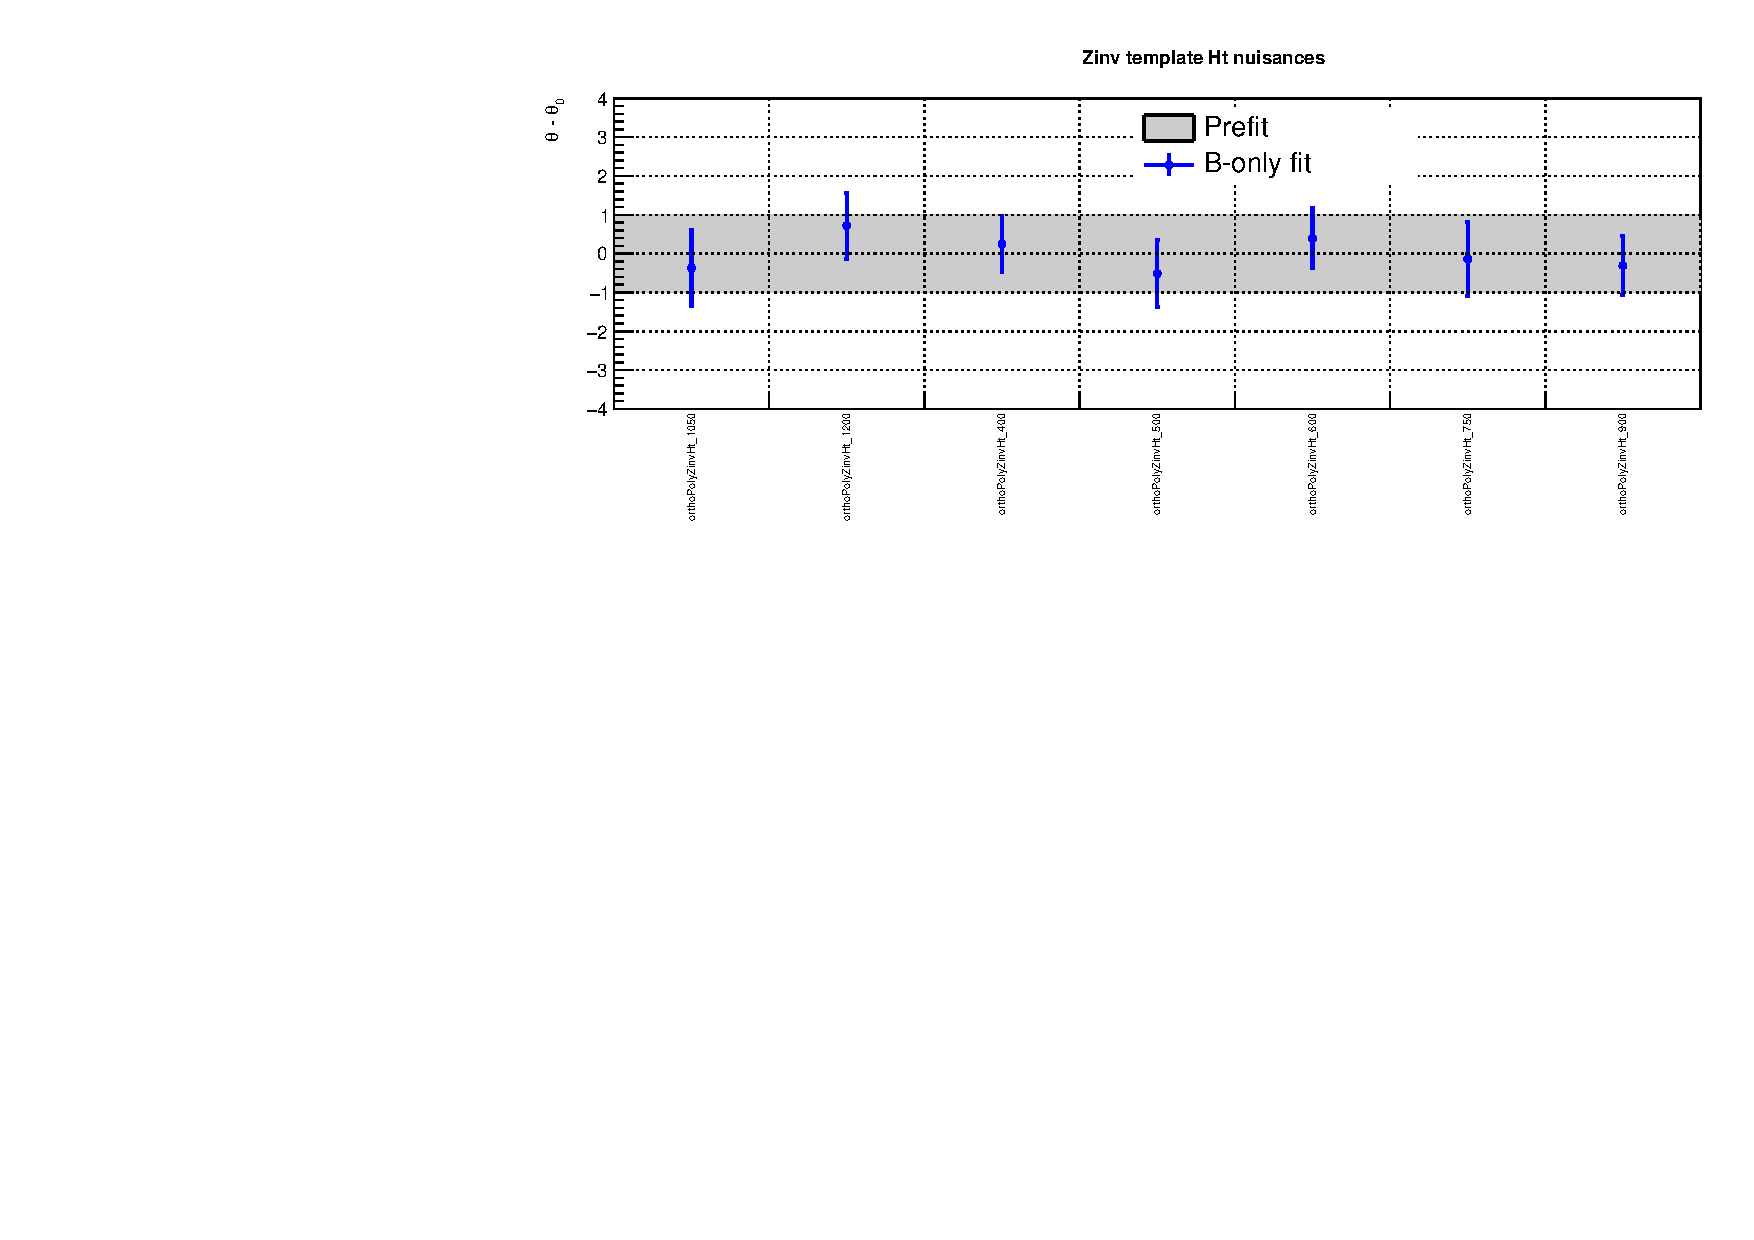
\includegraphics[width=1.\linewidth]{figures/results/postfit/nuis/TemplateZinv_ht_nuisances}
\end{figure}

\begin{figure}[h!]
  \centering
  \caption{Systematic uncertainties per \njet category in \mht modelling for \znunuj background}
  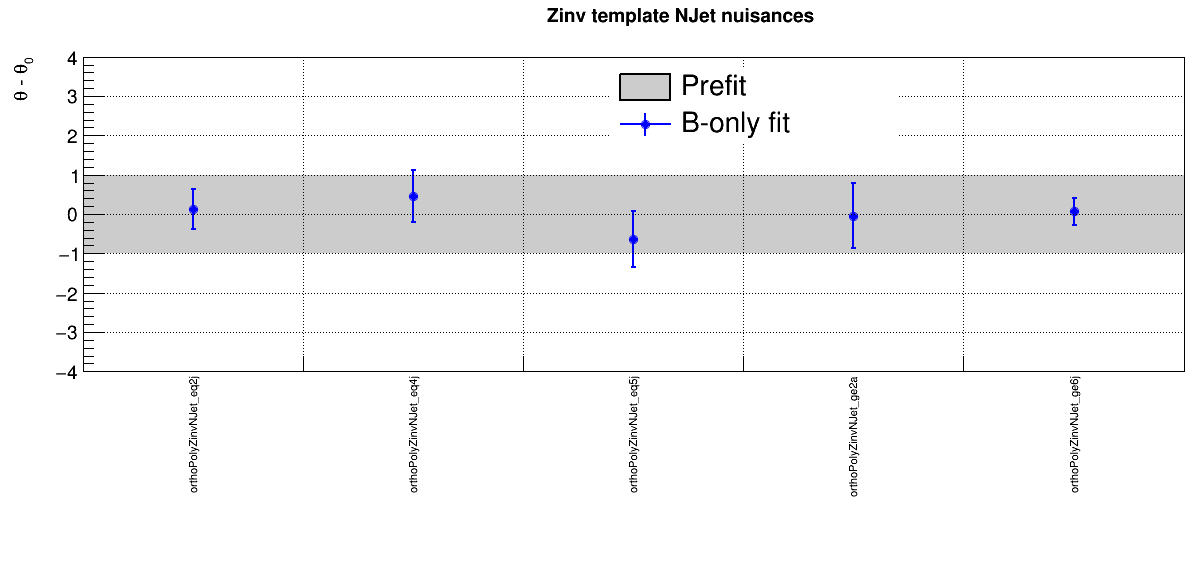
\includegraphics[width=1.\linewidth]{figures/results/postfit/nuis/TemplateZinv_njet_nuisances}
\end{figure}

\clearpage
\begin{figure}[h!]
  \centering
  \caption{Systematic uncertainties in \alphat modelling}
  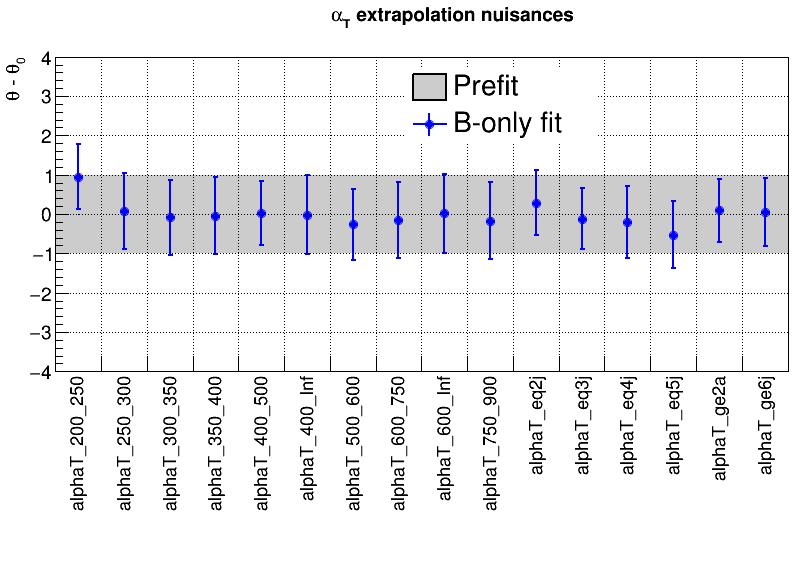
\includegraphics[width=0.8\linewidth]{figures/results/postfit/nuis/AlphaT_nuisances}
\end{figure}

\begin{figure}[h!]
  \centering
  \caption{Systematic uncertainties in \bdphi modelling}
  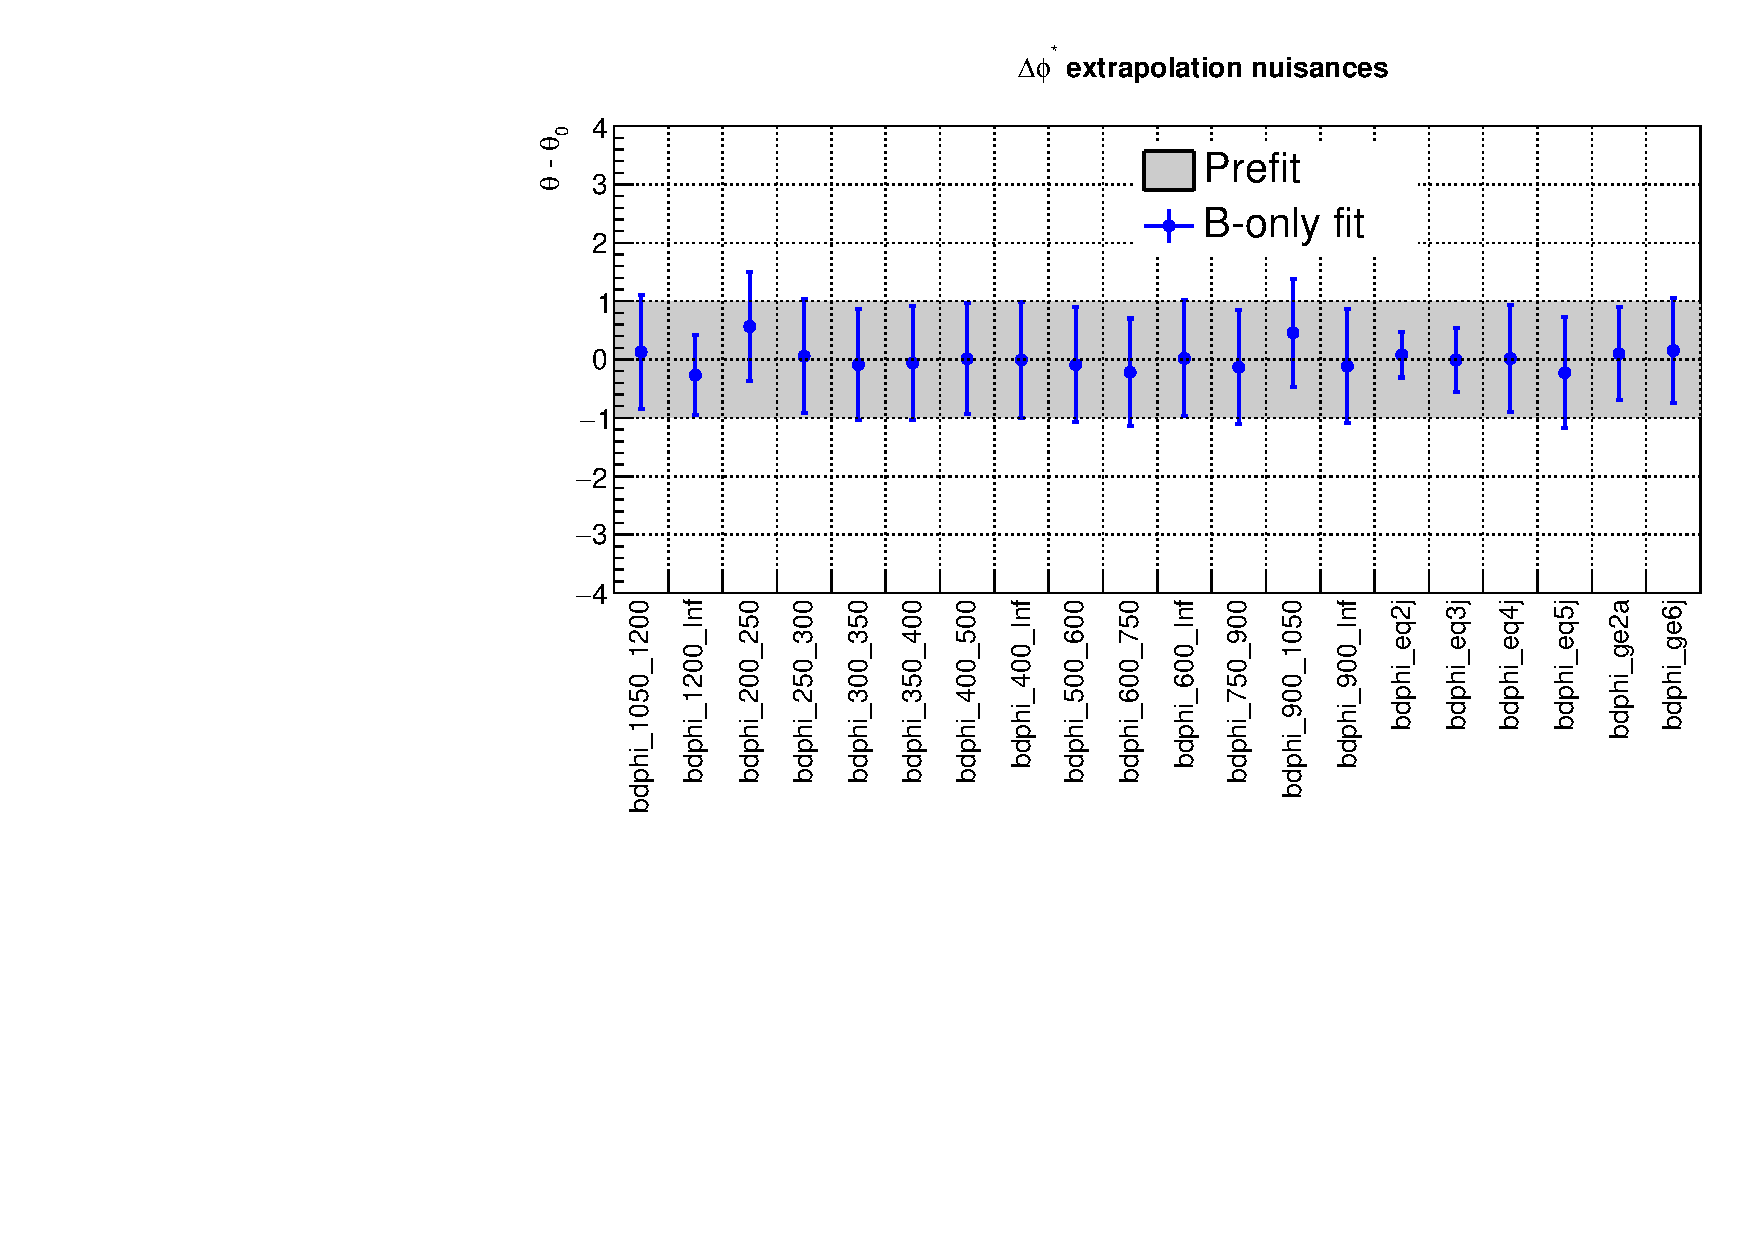
\includegraphics[width=0.8\linewidth]{figures/results/postfit/nuis/bDPhi_nuisances}
\end{figure}

\clearpage
\begin{figure}[h!]
  \centering
  \caption{Systematic uncertainties in single isolated track veto modelling}
  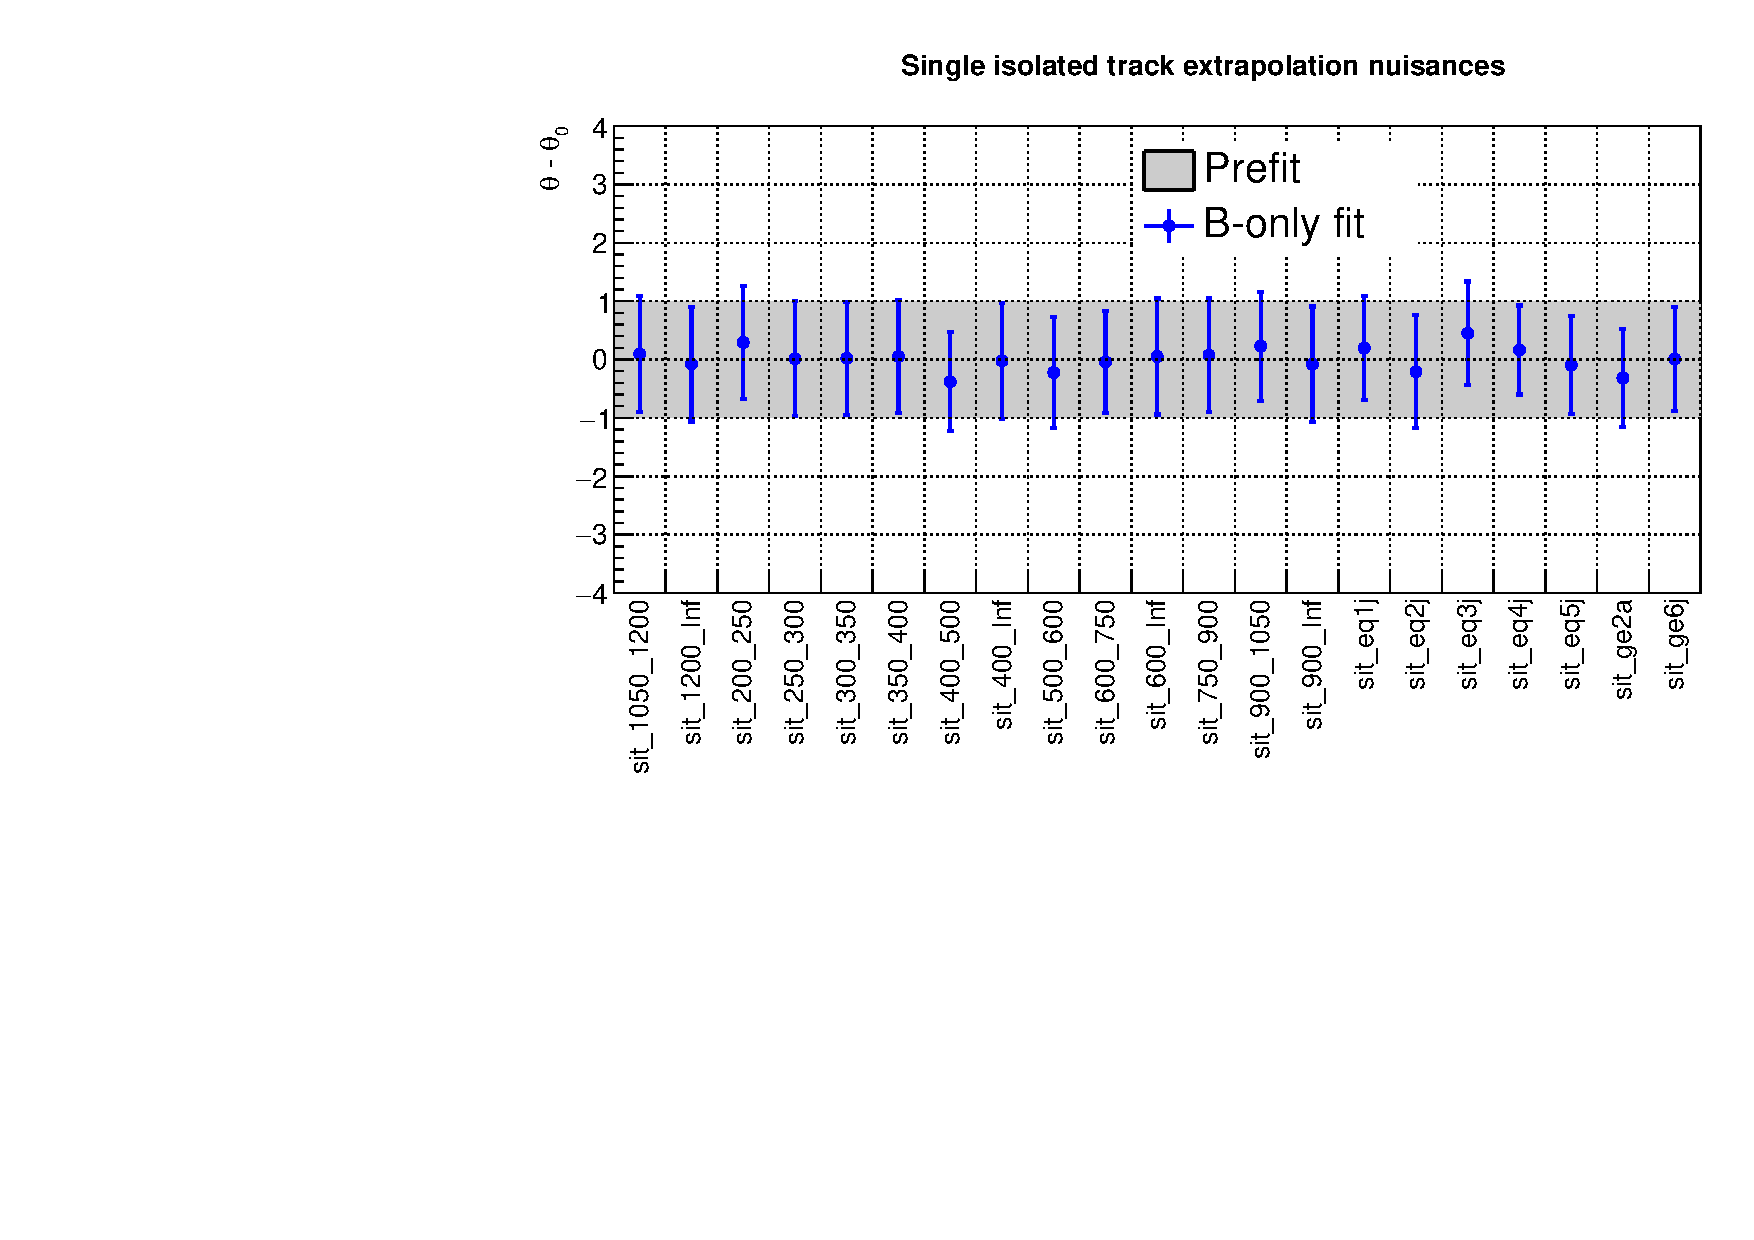
\includegraphics[width=0.8\linewidth]{figures/results/postfit/nuis/SIT_nuisances}
\end{figure}

\begin{figure}[h!]
  \centering
  \caption{Systematic uncertainties in W polarisation modelling}
  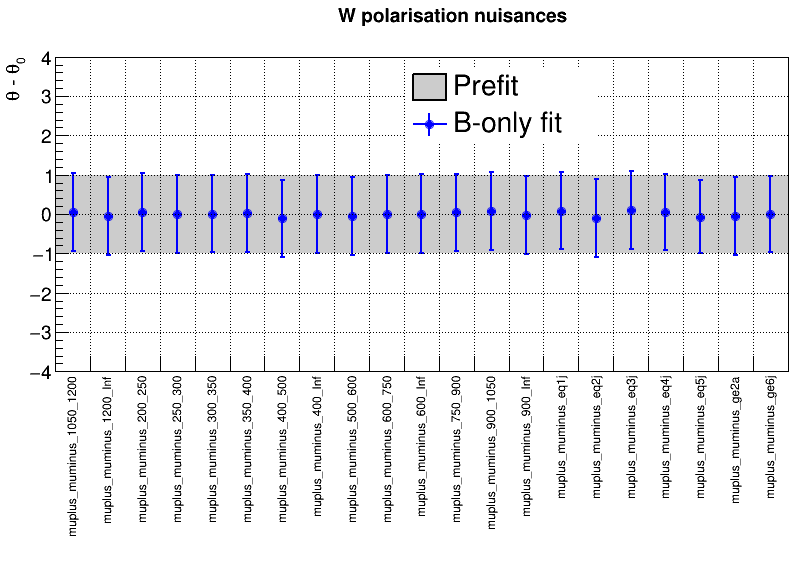
\includegraphics[width=0.8\linewidth]{figures/results/postfit/nuis/WPol_nuisances}
\end{figure}

